	
%% bare_conf.tex
%% V1.4b
%% 2015/08/26
%% by Michael Shell
%% See:
%% http://www.michaelshell.org/
%% for current contact information.
%%
%% This is a skeleton file demonstrating the use of IEEEtran.cls
%% (requires IEEEtran.cls version 1.8b or later) with an IEEE
%% conference paper.
%%
%% Support sites:
%% http://www.michaelshell.org/tex/ieeetran/
%% http://www.ctan.org/pkg/ieeetran
%% and
%% http://www.ieee.org/

%%*************************************************************************
%% Legal Notice:
%% This code is offered as-is without any warranty either expressed or
%% implied; without even the implied warranty of MERCHANTABILITY or
%% FITNESS FOR A PARTICULAR PURPOSE! 
%% User assumes all risk.
%% In no event shall the IEEE or any contributor to this code be liable for
%% any damages or losses, including, but not limited to, incidental,
%% consequential, or any other damages, resulting from the use or misuse
%% of any information contained here.
%%
%% All comments are the opinions of their respective authors and are not
%% necessarily endorsed by the IEEE.
%%
%% This work is distributed under the LaTeX Project Public License (LPPL)
%% ( http://www.latex-project.org/ ) version 1.3, and may be freely used,
%% distributed and modified. A copy of the LPPL, version 1.3, is included
%% in the base LaTeX documentation of all distributions of LaTeX released
%% 2003/12/01 or later.
%% Retain all contribution notices and credits.
%% ** Modified files should be clearly indicated as such, including  **
%% ** renaming them and changing author support contact information. **
%%*************************************************************************


% *** Authors should verify (and, if needed, correct) their LaTeX system  ***
% *** with the testflow diagnostic prior to trusting their LaTeX platform ***
% *** with production work. The IEEE's font choices and paper sizes can   ***
% *** trigger bugs that do not appear when using other class files.       ***                          ***
% The testflow support page is at:
% http://www.michaelshell.org/tex/testflow/



\documentclass[conference]{IEEEtran}
% Some Computer Society conferences also require the compsoc mode option,
% but others use the standard conference format.
%
% If IEEEtran.cls has not been installed into the LaTeX system files,
% manually specify the path to it like:
% \documentclass[conference]{../sty/IEEEtran}





% Some very useful LaTeX packages include:
% (uncomment the ones you want to load)


% *** MISC UTILITY PACKAGES ***
%
%\usepackage{ifpdf}
% Heiko Oberdiek's ifpdf.sty is very useful if you need conditional
% compilation based on whether the output is pdf or dvi.
% usage:
% \ifpdf
%   % pdf code
% \else
%   % dvi code
% \fi
% The latest version of ifpdf.sty can be obtained from:
% http://www.ctan.org/pkg/ifpdf
% Also, note that IEEEtran.cls V1.7 and later provides a builtin
% \ifCLASSINFOpdf conditional that works the same way.
% When switching from latex to pdflatex and vice-versa, the compiler may
% have to be run twice to clear warning/error messages.






% *** CITATION PACKAGES ***
%
%\usepackage{cite}
% cite.sty was written by Donald Arseneau
% V1.6 and later of IEEEtran pre-defines the format of the cite.sty package
% \cite{} output to follow that of the IEEE. Loading the cite package will
% result in citation numbers being automatically sorted and properly
% "compressed/ranged". e.g., [1], [9], [2], [7], [5], [6] without using
% cite.sty will become [1], [2], [5]--[7], [9] using cite.sty. cite.sty's
% \cite will automatically add leading space, if needed. Use cite.sty's
% noadjust option (cite.sty V3.8 and later) if you want to turn this off
% such as if a citation ever needs to be enclosed in parenthesis.
% cite.sty is already installed on most LaTeX systems. Be sure and use
% version 5.0 (2009-03-20) and later if using hyperref.sty.
% The latest version can be obtained at:
% http://www.ctan.org/pkg/cite
% The documentation is contained in the cite.sty file itself.






% *** GRAPHICS RELATED PACKAGES ***
%
\ifCLASSINFOpdf
  % \usepackage[pdftex]{graphicx}
  % declare the path(s) where your graphic files are
  % \graphicspath{{../pdf/}{../jpeg/}}
  % and their extensions so you won't have to specify these with
  % every instance of \includegraphics
  % \DeclareGraphicsExtensions{.pdf,.jpeg,.png}
\else
  % or other class option (dvipsone, dvipdf, if not using dvips). graphicx
  % will default to the driver specified in the system graphics.cfg if no
  % driver is specified.
  % \usepackage[dvips]{graphicx}
  % declare the path(s) where your graphic files are
  % \graphicspath{{../eps/}}
  % and their extensions so you won't have to specify these with
  % every instance of \includegraphics
  % \DeclareGraphicsExtensions{.eps}
\fi
% graphicx was written by David Carlisle and Sebastian Rahtz. It is
% required if you want graphics, photos, etc. graphicx.sty is already
% installed on most LaTeX systems. The latest version and documentation
% can be obtained at: 
% http://www.ctan.org/pkg/graphicx
% Another good source of documentation is "Using Imported Graphics in
% LaTeX2e" by Keith Reckdahl which can be found at:
% http://www.ctan.org/pkg/epslatex
%
% latex, and pdflatex in dvi mode, support graphics in encapsulated
% postscript (.eps) format. pdflatex in pdf mode supports graphics
% in .pdf, .jpeg, .png and .mps (metapost) formats. Users should ensure
% that all non-photo figures use a vector format (.eps, .pdf, .mps) and
% not a bitmapped formats (.jpeg, .png). The IEEE frowns on bitmapped formats
% which can result in "jaggedy"/blurry rendering of lines and letters as
% well as large increases in file sizes.
%
% You can find documentation about the pdfTeX application at:
% http://www.tug.org/applications/pdftex





% *** MATH PACKAGES ***
%
%\usepackage{amsmath}
% A popular package from the American Mathematical Society that provides
% many useful and powerful commands for dealing with mathematics.
%
% Note that the amsmath package sets \interdisplaylinepenalty to 10000
% thus preventing page breaks from occurring within multiline equations. Use:
%\interdisplaylinepenalty=2500
% after loading amsmath to restore such page breaks as IEEEtran.cls normally
% does. amsmath.sty is already installed on most LaTeX systems. The latest
% version and documentation can be obtained at:
% http://www.ctan.org/pkg/amsmath





% *** SPECIALIZED LIST PACKAGES ***
%
%\usepackage{algorithmic}
% algorithmic.sty was written by Peter Williams and Rogerio Brito.
% This package provides an algorithmic environment fo describing algorithms.
% You can use the algorithmic environment in-text or within a figure
% environment to provide for a floating algorithm. Do NOT use the algorithm
% floating environment provided by algorithm.sty (by the same authors) or
% algorithm2e.sty (by Christophe Fiorio) as the IEEE does not use dedicated
% algorithm float types and packages that provide these will not provide
% correct IEEE style captions. The latest version and documentation of
% algorithmic.sty can be obtained at:
% http://www.ctan.org/pkg/algorithms
% Also of interest may be the (relatively newer and more customizable)
% algorithmicx.sty package by Szasz Janos:
% http://www.ctan.org/pkg/algorithmicx




% *** ALIGNMENT PACKAGES ***
%
%\usepackage{array}
% Frank Mittelbach's and David Carlisle's array.sty patches and improves
% the standard LaTeX2e array and tabular environments to provide better
% appearance and additional user controls. As the default LaTeX2e table
% generation code is lacking to the point of almost being broken with
% respect to the quality of the end results, all users are strongly
% advised to use an enhanced (at the very least that provided by array.sty)
% set of table tools. array.sty is already installed on most systems. The
% latest version and documentation can be obtained at:
% http://www.ctan.org/pkg/array


% IEEEtran contains the IEEEeqnarray family of commands that can be used to
% generate multiline equations as well as matrices, tables, etc., of high
% quality.




% *** SUBFIGURE PACKAGES ***
%\ifCLASSOPTIONcompsoc
%  \usepackage[caption=false,font=normalsize,labelfont=sf,textfont=sf]{subfig}
%\else
%  \usepackage[caption=false,font=footnotesize]{subfig}
%\fi
% subfig.sty, written by Steven Douglas Cochran, is the modern replacement
% for subfigure.sty, the latter of which is no longer maintained and is
% incompatible with some LaTeX packages including fixltx2e. However,
% subfig.sty requires and automatically loads Axel Sommerfeldt's caption.sty
% which will override IEEEtran.cls' handling of captions and this will result
% in non-IEEE style figure/table captions. To prevent this problem, be sure
% and invoke subfig.sty's "caption=false" package option (available since
% subfig.sty version 1.3, 2005/06/28) as this is will preserve IEEEtran.cls
% handling of captions.
% Note that the Computer Society format requires a larger sans serif font
% than the serif footnote size font used in traditional IEEE formatting
% and thus the need to invoke different subfig.sty package options depending
% on whether compsoc mode has been enabled.
%
% The latest version and documentation of subfig.sty can be obtained at:
% http://www.ctan.org/pkg/subfig




% *** FLOAT PACKAGES ***
%
%\usepackage{fixltx2e}
% fixltx2e, the successor to the earlier fix2col.sty, was written by
% Frank Mittelbach and David Carlisle. This package corrects a few problems
% in the LaTeX2e kernel, the most notable of which is that in current
% LaTeX2e releases, the ordering of single and double column floats is not
% guaranteed to be preserved. Thus, an unpatched LaTeX2e can allow a
% single column figure to be placed prior to an earlier double column
% figure.
% Be aware that LaTeX2e kernels dated 2015 and later have fixltx2e.sty's
% corrections already built into the system in which case a warning will
% be issued if an attempt is made to load fixltx2e.sty as it is no longer
% needed.
% The latest version and documentation can be found at:
% http://www.ctan.org/pkg/fixltx2e


%\usepackage{stfloats}
% stfloats.sty was written by Sigitas Tolusis. This package gives LaTeX2e
% the ability to do double column floats at the bottom of the page as well
% as the top. (e.g., "\begin{figure*}[!b]" is not normally possible in
% LaTeX2e). It also provides a command:
%\fnbelowfloat
% to enable the placement of footnotes below bottom floats (the standard
% LaTeX2e kernel puts them above bottom floats). This is an invasive package
% which rewrites many portions of the LaTeX2e float routines. It may not work
% with other packages that modify the LaTeX2e float routines. The latest
% version and documentation can be obtained at:
% http://www.ctan.org/pkg/stfloats
% Do not use the stfloats baselinefloat ability as the IEEE does not allow
% \baselineskip to stretch. Authors submitting work to the IEEE should note
% that the IEEE rarely uses double column equations and that authors should try
% to avoid such use. Do not be tempted to use the cuted.sty or midfloat.sty
% packages (also by Sigitas Tolusis) as the IEEE does not format its papers in
% such ways.
% Do not attempt to use stfloats with fixltx2e as they are incompatible.
% Instead, use Morten Hogholm'a dblfloatfix which combines the features
% of both fixltx2e and stfloats:
%
% \usepackage{dblfloatfix}
% The latest version can be found at:
% http://www.ctan.org/pkg/dblfloatfix




% *** PDF, URL AND HYPERLINK PACKAGES ***
%
%\usepackage{url}
% url.sty was written by Donald Arseneau. It provides better support for
% handling and breaking URLs. url.sty is already installed on most LaTeX
% systems. The latest version and documentation can be obtained at:
% http://www.ctan.org/pkg/url
% Basically, \url{my_url_here}.




% *** Do not adjust lengths that control margins, column widths, etc. ***
% *** Do not use packages that alter fonts (such as pslatex).         ***
% There should be no need to do such things with IEEEtran.cls V1.6 and later.
% (Unless specifically asked to do so by the journal or conference you plan
% to submit to, of course. )


% correct bad hyphenation here
\hyphenation{op-tical net-works semi-conduc-tor}
\usepackage{graphicx}
\usepackage{array}
\usepackage{filecontents}
\usepackage{caption}
\usepackage[noadjust]{cite}
\captionsetup[table]{position=bottom}   %% or below

\begin{document}
%
% paper title
% Titles are generally capitalized except for words such as a, an, and, as,
% at, but, by, for, in, nor, of, on, or, the, to and up, which are usually
% not capitalized unless they are the first or last word of the title.
% Linebreaks \\ can be used within to get better formatting as desired.
% Do not put math or special symbols in the title.
\title{Precise Weed and Maize classification through Convolutional Neuronal Networks }


% author names and affiliations
% use a multiple column layout for up to three different
% affiliations
\author{\IEEEauthorblockN{Andrea Concepci\'on C\'ordova Cruzatty \IEEEauthorrefmark{1},
Mauricio Daniel Barreno Barreno \IEEEauthorrefmark{2} and Jos\'e Misael J\'acome Barrionuevo\IEEEauthorrefmark{3}}
\IEEEauthorblockA{Department of Energy and Mechanics,
University of the Army ESPE\\
Latacunga - Quijano y Ordo\~nez and Hermanas Pa\'ez \\
Email: \IEEEauthorrefmark{1}accordova@espe.edu.ec,
\IEEEauthorrefmark{2}mdbarreno@espe.edu.ec,
\IEEEauthorrefmark{3}jmjacome1@espe.edu.ec}}
% conference papers do not typically use \thanks and this command
% is locked out in conference mode. If really needed, such as for
% the acknowledgment of grants, issue a \IEEEoverridecommandlockouts
% after \documentclass

% for over three affiliations, or if they all won't fit within the width
% of the page, use this alternative format:
% 
%\author{\IEEEauthorblockN{Michael Shell\IEEEauthorrefmark{1},
%Homer Simpson\IEEEauthorrefmark{2},
%James Kirk\IEEEauthorrefmark{3}, 
%Montgomery Scott\IEEEauthorrefmark{3} and
%Eldon Tyrell\IEEEauthorrefmark{4}}
%\IEEEauthorblockA{\IEEEauthorrefmark{1}School of Electrical and Computer Engineering\\
%Georgia Institute of Technology,
%Atlanta, Georgia 30332--0250\\ Email: see http://www.michaelshell.org/contact.html}
%\IEEEauthorblockA{\IEEEauthorrefmark{2}Twentieth Century Fox, Springfield, USA\\
%Email: homer@thesimpsons.com}
%\IEEEauthorblockA{\IEEEauthorrefmark{3}Starfleet Academy, San Francisco, California 96678-2391\\
%Telephone: (800) 555--1212, Fax: (888) 555--1212}
%\IEEEauthorblockA{\IEEEauthorrefmark{4}Tyrell Inc., 123 Replicant Street, Los Angeles, California 90210--4321}}




% use for special paper notices
%\IEEEspecialpapernotice{(Invited Paper)}




% make the title area
\maketitle

% As a general rule, do not put math, special symbols or citations
% in the abstract
\begin{abstract}
Deep Learning has played a very important role in modern times, being very used in Artificial Vision and especially in Pattern Recognition, which opens many doors in the fields of application among which is precision agriculture. In this paper we present the study of a convolutional neural network with two classes applied to the classification of plants of maize and weeds in real time, focused to fields of maize in its initial stage. The algorithm has two stages, segmentation of images and classification.  In the segmentation we wanted to separate the target plant from the original image. While the classification is possible through a convolutional neural network, previously trained with a dataset generated through the segmentation stage. The performance of the network is illustrated by analysis and comparisons with different network architectures, then with the network that presented better results in training, we experimented by modifying its number of filters, to analyze their  behavior. Finally, the resulting network was tested on different processors to compare classification times.\\
\end{abstract}

% no keywords




% For peer review papers, you can put extra information on the cover
% page as needed:
% \ifCLASSOPTIONpeerreview
% \begin{center} \bfseries EDICS Category: 3-BBND \end{center}
% \fi
%
% For peerreview papers, this IEEEtran command inserts a page break and
% creates the second title. It will be ignored for other modes.
\IEEEpeerreviewmaketitle

\section{Introduction}
During the last centuries, huge progress has taken place in science and technology developments. Significant milestones such as Communications, Numerical Computer Control and the miniaturization of components have benefited social and industrial sectors on its approach to solve specific problems. 
\\

Globalization has permitted countries who are not leader technology developers, like Ecuador, to receive bleeding edge technological products in order to satisfy requirements and propose solutions to still-unresolved problems.
\\

Industry transformation is a science evolution example; manufacturing, food, and information industries, among others, are signs of this industrial revolution. However there are fields still unexplored  in Ecuador like agroindustry. Agriculture in Ecuador has not changed much since precolombine times; while it is true that there are efficient agriculture practices, the lack of technological resources make it impossible for the country to exploit its true potential as an agricultural producer.
\\

Nowadays, one of agriculture challenges is the development of precision agriculture techniques focused on Weed and Crop segmentation. There are studies that show the impact of Weed in corn crops \cite{suarez2005distintos}; its yield is affected by 5000 kg/ha. Currently, growing development of Artificial Vision and Machine Learning algorithms allow researchers to propose solutions for Weed Segmentation in Crops. 
\\

One of the first approximations to the algorithms of detection of Crops was  developed in 1996 \cite{brivot1996segmentation}, this algorithm permitted to segment crops from weed, it could be possible by the use of IR Images, the image is processed by a hysteresis umbral and the method of Min Neighbouring to identify the row of crops. In recent years the implementation of Machine Learning has opened new possibilities for differentiate the Weed from the crops, recently \cite{cheng2015feature} there had been developed an algorithm by the use of Harris Corner detector, Feature Detector and using the DBSCAN (Density-based spartial clustering of apllications with noise) , it demonstrates an effectiveness of  98\% in the identification of Weeds in the Rice, Araguez \textit{et. al} \cite{equipo2006proceedings}  performed their segmentation through the analysis of the green hystogram and performing the segmentation of the crop and weed by classifiers not specified in the document. 
\\

Hong and Lei \cite{jeon2011robust} developed their approximation by using an optimal method for detection in various types of luminosity, they achived this by the use an ANN for weed and maize classification, with a precision of 92.5\%,  also there had been developed an algorithm \cite{hlaing2014weed}, that through binarization methods of OTSU and Watershed for the segmentation of the images. While its classification was given through an areas analysis to perform a thresholding, although the method is computationally effective when the Weed distribution does not resemble the size to the crop plant, its error increases when there is more density of crop than of weed. Romeo \textit{et. al} \cite{romeo2012crop} propose to use a fuzzy clustering approach to correctly segment the crop green.
\\

The segmentation of weed and crops is not closed to color images, using a multispectral camera  \cite{potena2016fast} permitted to obtain RGB and NIR images, for the segmentation and classification, then the images used a light CNN for the first process and a Deep CNN for classification in Crops, its accuracy is up to 98\% in the identification of weeds. One of the most dificults things for the identification of crops is the generation of Datasets due to presence of Weed in the images of training, but there could be correctly generated by a Convolutional Neural Network \cite{di2016automatic} achieving a acceptable accuracy for the generation of Datasets. 
\\

\section{Matherials and Methods}
The development of the model for the weed and maize detection algorithm using convolutional neural networks is described below.
\\
\subsection{Hardware}
For the training and image capturing stages, the following elements were used: a Raspberry Pi 3 with Pi Camera V2.1 for image acquisition, it was configured to obtain a video at a resolution of 1280x720 pixels in order to get more detail in the segmented images. Due to the popularity of the GPU computing, it was neccesary to consider hardware compatible with Parallel Computing like the Graphic Cards manufactured by NVIDIA, they have the advantage of better times of processing compared to CPU, in order to optimize the time of image processing and training of Deep Learning Models, so we used a Computer with a Nvidia Graphics Card GTX950M. Also it was neccesary to consider the use of a CPU Core i7 2.7 Ghz, 8 cores and the CPU of the Raspberry Pi 3, a ARM Cortex-A53, 1.2GHz, 4 cores for testing the classification of images of the Network.   
\\

\subsection{Software}

For the application in this documents it requires the use of powerful libraries of Image Processing and Deep Learning Development, we considered to use Open Software for extend its use in future prototypes, due to this considerations we had chosen the OpenCV library for its computational efficiency and focus on real-time application \cite{opencv_library} in this  case, it was used for acquisition and segmentation of the sample images. Also we had considered Caffe because it is intended to use in training and developing general-purpose Convolutionals Neural Networks and other Deep Lerning models \cite{jia2014caffe} with fully support of CUDA GPU Computation and a generous database of resources for learning,	
\\

Also in the development stage was important the use of Linux OS , its features are: lightweight and free OS also fully compatible with the software mentioned above. For the main computer was used Ubuntu Linux 16.04 for its official support to CUDA, Caffe and OpenCV, also in the Raspberry Pi we used the Pixel OS for acquire images and processing of the CNN.
\\

\subsection{Dataset Description}
Due to the lack of datasets of Weed and Maize plants, it was neccesary to search crops of maize in its initial stage, for that purpose we had traslated to P\'illaro, it is a city located in the Tungurahua Province on the center of the Ecuadorian Highlands region, P\'illaro is recognized producer of Andean Crops such as: Maize, Potatoes and Fruits so here we could find many crops of Maize useful for our purpose. \\


Samples were obtained from images captured in those maize fields , we considered to choose maize crops where we could visually discriminate the plants of the crop and the weed. Maize in stages V3-V7(3-7 leafs) \cite{fassio1998maiz} were used to take samples. To record the samples we centered the camera over the target plant, insuring that the capture shows all features of the maize plant, it was possible by monitoring the get of samples by an external display. An examples of the images captured are shown below. 


	\begin{figure}[h]
	\centering
	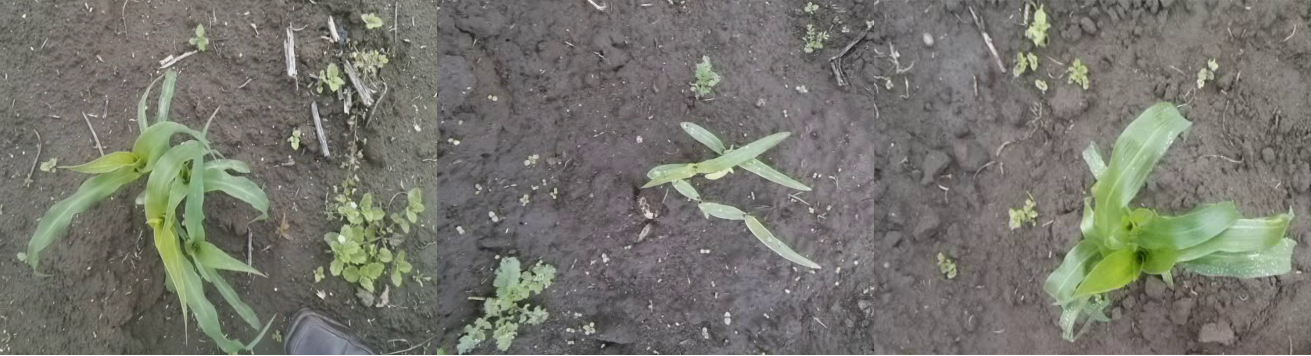
\includegraphics[width=3.2in]{entradamaiz}
	\caption{Crops chosen to obtain samples, notice that it is easy to discrimante weed from maize}
	\label{fig_sim}
	\end{figure}

Also it was neccesary  to obtain images of the most common weed plants of the maize crops in Pillaro, to allow the Network to discriminate both classes of the Dataset. \\
	
Then, through a digital image processing, the images were segmented to differentiate them from the soil and other non-plant elements, then the images were masked to provide the dataset features of color of the Maize and Weed. Once the segmented images were obtained, they were removed those that had a resolution lower than 64x64 pixels, because it's smaller than size of input layer of the network, besides it was not convenient its processing since its total area was much smaller than the samples of corn, which is the purpose of this document, later, the images were saved in a png format. The process described before, was illustrated in the next figure. \\
	\begin{figure}[h]
	\centering
	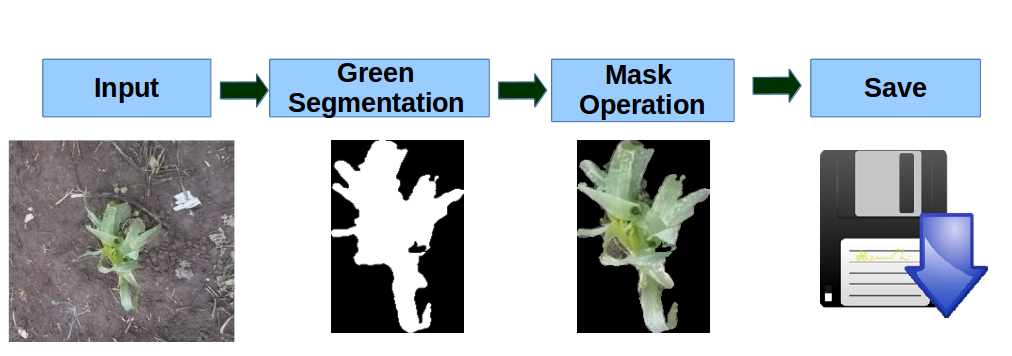
\includegraphics[width=3.2in]{procesamiento}
	\caption{Preprocessing to obtain samples for the dataset}
	\label{fig_sim}
	\end{figure}
	
To highlight we had labelled the samples manually in two classes. In the following image we present the final results of the processed images that conform the dataset.\\
	
	\begin{figure}[h]
	\centering
	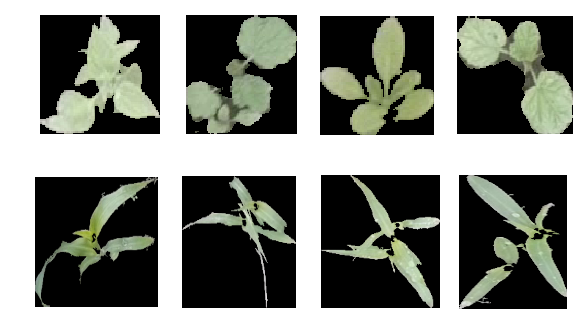
\includegraphics[width=2.5in]{im1}
	\caption{ Segmented and Masked images of dataset Above: Weed, Below: Maize}
	\label{fig_sim}
	\end{figure}
	
Once we completed the processing of the images, it were obtained 2835 images of Maize and 880 images of Weed, Lee \textit{et. al} \cite{lee2015deep} said that once CNN has reached an acceptable accuracy, the dataset could extend by Geometric Transformations, in addition \cite{sladojevic2016deep}  they mention that this allows to reduce the overfitting and to improve the precision in the training, reason why we made 11 rotations each 30 degrees, obtaining in this way to increase the dataset in 12 times and have better chances of recognizing plants that are in any orientation. \\

For the Validation Phase, we had chosen randomly a fifth part of the total images of each class, so we have the following chart with the distribution of the dataset.

\begin{table}[h!]
\centering
\begin{tabular}{| c | c | c | c | c |} 
 \hline
 Phase & Train & Validation & Test & Total \\ [1ex] 
 \hline
 Maize & 25695 & 8325 & 200 & 34220  \\ 
 Weed & 8560 & 2000 & 200 & 10760\\ 
 \hline
\end{tabular}
\caption{Distribution of the Dataset of each class}
\label{table:1}
\end{table}
	
	
\subsection{Convolutional Neuronal Network}
	After the last step have been terminated, it is neccesary classify the images of Maize and Weed, a high accurate method of Image Classification is Convolutional Neuronal Networks(CNN), those models are complex but efficient with a highly rate of discrimination and its demostrated that they have good results in Image Classification, Object Detection and Fine-Grained  Classification \cite{sharif2014cnn}. Their are also applied in Precision Agriculture \cite{potena2016fast} for the correct identification of plants.
\\ 

One of the characteristics of the CNN is that they can have multiple architectures, each architecture can reach different result depending of the application , for the present document we have considered four CNN architectures: Two models were chose of the Caffe Zoo Model(it's a free resource provided by Caffe Developers), LeNet and AlexNet also Potena and Nardi had used two additional types of Models, sNET and cNET, they were sucessfully proved in identification of plants in crops\cite{potena2016fast}, with the Nets chosen, each one was trained with a same Solver of type AdaDelta and with the same dataset, the results of training are the following. \\
\begin{table}[h!]
\centering
\begin{tabular}{|l c c c c|} 
 \hline
 Parameters & LeNet & AlexNet & cNET & sNET \\ [0.75ex] 
 \hline
 Input size of images & 32x32 & 64x64 & 64x64 & 64x64 \\ 
 Layers numbers & 9 & 11 & 8 & 4\\
 Number of parameters & 652500 & 20166688 & 6421568 & 135872 \\ 
 Iterations & 3000 & 3000 & 3000 & 3000 \\ 
  Accuracy(\%) & 86.48 & 93.86 & 95.33 & 80.4 \\
  Loss(\%) & 32.80 & 15.32 & 13.72 & 15.32 \\ [1ex] 
 \hline 
\end{tabular}
\caption{Distribution of the Dataset of each class}
\label{table:2}
\end{table}

Inside of the shown parameters in the Table \ref{table:2}, we considered the net who achieved the highest rate of accuracy and lowest rate of loss, clearly the cNET is the chosen due it shows a precission near to human classification.\\
	
Although results given for the net are excellents, one of the main purposes of this paper is the implementation in real time, so the number of parameters to be computed must be a problem, so we considered to modify the net in order to improve the processing time. To achive this, it was neccesary to reduce the number of filters of cNET from 64 to 16.\\

\begin{table}[h!]
\centering
\begin{tabular}{|l c c |} 
 \hline
 Parameters & cNET 16 filters & cNET 64 filters \\ [0.75ex] 
 \hline
 Number of parameters & 1651376 & 6421568 \\ 
 Iterations & 9000 & 9000  \\ 
  Accuracy(\%) & 97.26 & 96.40  \\
  Loss(\%) & 8.39 & 14.48  \\ [1ex] 
 \hline 
\end{tabular}
\caption{Distribution of the Dataset of each class}
\label{table:3}
\end{table}

This permitted to reduce the number of parameters to 1651376(it's a 25\% of parameters than the original net), and what about the precision of the net, it was slighty affected but it reach a 97.2\% of accuracy.\\
	
	\begin{figure}[h]
	\centering
	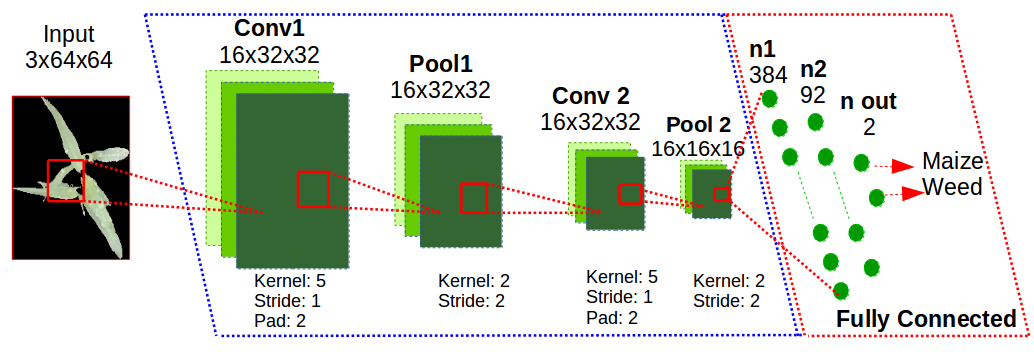
\includegraphics[width=3.6 in]{arquitectura}
	\caption{ The schematic of CNet }
	\label{fig_sim}
	\end{figure}
	
	\begin{figure}[h]
	\centering
	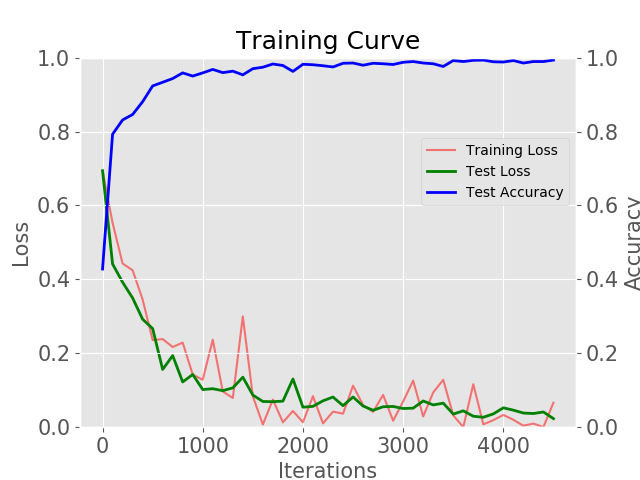
\includegraphics[width=2.4in]{entrenamiento}
	\caption{ Graph of the Training Process }
	\label{fig_sim}
	\end{figure}
	
The before pictures shows the schematic of the cNET of 16 filters and its process of training.Note that by reducing the number of filters the network gained accuracy because it does not have so much data to process.\\

	\section{Test}

For this stage, we considered an extra dataset with 200 images of maize plants in stage of V3-V7 and 203 images of weed, obtained in maize crops, the results were comparated between cNET with 64 and 16 filters in the Table \ref{table:4}.\\  
\begin{table}[h!]
\centering
\begin{tabular}{|l|c|c|p{2cm}|}  
 \hline
 \multicolumn{4}{ |c| }{GPU} \\
 \hline
   cNET & \% Accuracy Weed & \% Accuracy Maize  & Average time of classification   \\ 
 \hline 
 64 Filters & 81.6 & 88.36 & 2.34 ms  \\ [0.75ex]
 \hline
 16 Filters & 85.71 & 87.13 & 951  $\mu$ s \\ [0.75ex]
  \hline
 \multicolumn{4}{ |c| }{CPU} \\
 \hline
   & \% Accuracy Weed & \%Accuracy Maize  & Average time of classification \\ 
 \hline 
 64 Filters & 81.6 & 88.36 & 51.6 ms  \\ [0.75ex]
 \hline
 16 Filters & 85.71 & 87.13 & 17.23 ms \\ [0.75ex]
  \hline
 \multicolumn{4}{ |c| }{CPU Raspberry Pi 3} \\
 \hline
   & \% Accuracy Weed & \%Accuracy Maize  & Average time of classification\\ 
 \hline 
 64 Filters & 81.6 & 88.36 & 615 ms  \\ [0.75ex]
 \hline
 16 Filters & 85.71 & 87.13 & 161 s \\ [0.75ex]
  \hline
\end{tabular}
\caption{Test}
\label{table:4}
\end{table}

Like the table shown the results were achieved by the GPU processor, it is the best option to classificate a large amount of images however this project is thought to be portable, so we consider the RaspBerry Pi for the analysis of performance. With cNET of 64 filters the results fo time of classification was 615 miliseconds, so it time isn\'t the optimum for our objective that it is the processing in a real time.\\
	
	
	% An example of a floating figure using the graphicx package.
	% Note that \label must occur AFTER (or within) \caption.
	% For figures, \caption should occur after the \includegraphics.
	% Note that IEEEtran v1.7 and later has special internal code that
	% is designed to preserve the operation of \label within \caption
	% even when the captionsoff option is in effect. However, because
	% of issues like this, it may be the safest practice to put all your
	% \label just after \caption rather than within \caption{}.
	%
	% Reminder: the "draftcls" or "draftclsnofoot", not "draft", class
	% option should be used if it is desired that the figures are to be
	% displayed while in draft mode.
	%
	%\begin{figure}[!t]
	%\centering
	%\includegraphics[width=2.5in]{myfigure}
	% where an .eps filename suffix will be assumed under latex, 
	% and a .pdf suffix will be assumed for pdflatex; or what has been declared
	% via \DeclareGraphicsExtensions.
	%\caption{Simulation results for the network.}
	%\label{fig_sim}
	%\end{figure}
	
	% Note that the IEEE typically puts floats only at the top, even when this
	% results in a large percentage of a column being occupied by floats.
	
	
	% An example of a double column floating figure using two subfigures.
	% (The subfig.sty package must be loaded for this to work.)
	% The subfigure \label commands are set within each subfloat command,
	% and the \label for the overall figure must come after \caption.
	% \hfil is used as a separator to get equal spacing.
	% Watch out that the combined width of all the subfigures on a 
	% line do not exceed the text width or a line break will occur.
	%
	%\begin{figure*}[!t]
	%\centering
	%\subfloat[Case I]{\includegraphics[width=2.5in]{box}%
	%\label{fig_first_case}}
	%\hfil
	%\subfloat[Case II]{\includegraphics[width=2.5in]{box}%
	%\label{fig_second_case}}
	%\caption{Simulation results for the network.}
	%\label{fig_sim}
	%\end{figure*}
	%
	% Note that often IEEE papers with subfigures do not employ subfigure
	% captions (using the optional argument to \subfloat[]), but instead will
	% reference/describe all of them (a), (b), etc., within the main caption.
	% Be aware that for subfig.sty to generate the (a), (b), etc., subfigure
	% labels, the optional argument to \subfloat must be present. If a
	% subcaption is not desired, just leave its contents blank,
	% e.g., \subfloat[].
	
	
	% An example of a floating table. Note that, for IEEE style tables, the
	% \caption command should come BEFORE the table and, given that table
	% captions serve much like titles, are usually capitalized except for words
	% such as a, an, and, as, at, but, by, for, in, nor, of, on, or, the, to
	% and up, which are usually not capitalized unless they are the first or
	% last word of the caption. Table text will default to \footnotesize as
	% the IEEE normally uses this smaller font for tables.
	% The \label must come after \caption as always.
	%
	%\begin{table}[!t]
	%% increase table row spacing, adjust to taste
	%\renewcommand{\arraystretch}{1.3}
	% if using array.sty, it might be a good idea to tweak the value of
	% \extrarowheight as needed to properly center the text within the cells
	%\caption{An Example of a Table}
	%\label{table_example}
	%\centering
	%% Some packages, such as MDW tools, offer better commands for making tables
	%% than the plain LaTeX2e tabular which is used here.
	%\begin{tabular}{|c||c|}
	%\hline
	%One & Two\\
	%\hline
	%Three & Four\\
	%\hline
	%\end{tabular}
	%\end{table}
	
	
	% Note that the IEEE does not put floats in the very first column
	% - or typically anywhere on the first page for that matter. Also,
	% in-text middle ("here") positioning is typically not used, but it
	% is allowed and encouraged for Computer Society conferences (but
	% not Computer Society journals). Most IEEE journals/conferences use
	% top floats exclusively. 
	% Note that, LaTeX2e, unlike IEEE journals/conferences, places
	% footnotes above bottom floats. This can be corrected via the
	% \fnbelowfloat command of the stfloats package.




\section{Conclusion}

In this paper we have studied the application of Convolutional Neuronal Networks for Classification between Maize and Weed Plants, for that we have used some CNN Architectures, the Network with best results in precision was cNET, with a 99.33 \% of accuracy of training, using a dataset of both classes  of 44580 segmented images. \\

In order to search a right processing to work in real time, we have experimented to reduce the number of filters of the Layers of the Net from 64 to 16 filters, achiveiving to reduce the number of parameters to be computed during the classification , we obteined a classification time 2.5 times less than the original Net of 64 filters , this change had a small impact in the training accuray of the net, it value fell 1 \% in comparation with the original net. \\

Also, by using different methods to classify the images in our experiments, the results showed that the best time of classification was achieved by using a Nvidia Graphic Cards, this is due the Parallel Architecture that this GPU has and also it has fully support for the computation platform CUDA, it demostrated to be 18 times faster than a normal CPU and 170 times faster than a Raspberry Pi 3. \\

The study demostrated that is better to perform some geometrical tranformations to the Dataset images due it benefits to improve the  classification of plants because the plants ever have different orientations in the crop field. 




% conference papers do not normally have an appendix


% use section* for acknowledgment
\section*{Acknowledgment}

The authors would like to thank to the "Granja Agroecol\'ogica y Demostrativa" of P\'illaro City and owners of corn crops of the city which allowed us to take samples of plants, to obtain to conform the dataset of the project. \\

This work has been supported by the University of the Army "ESPE"  Latacunga.  


% trigger a \newpage just before the given reference
% number - used to balance the columns on the last page
% adjust value as needed - may need to be readjusted if
% the document is modified later
%\IEEEtriggeratref{8}
% The "triggered" command can be changed if desired:
%\IEEEtriggercmd{\enlargethispage{-5in}}

% references section

% can use a bibliography generated by BibTeX as a .bbl file
% BibTeX documentation can be easily obtained at:
% http://mirror.ctan.org/biblio/bibtex/contrib/doc/
% The IEEEtran BibTeX style support page is at:
% http://www.michaelshell.org/tex/ieeetran/bibtex/
%\bibliographystyle{IEEEtran}
% argument is your BibTeX string definitions and bibliography database(s)
%\bibliography{IEEEabrv,../bib/paper}
%
% <OR> manually copy in the resultant .bbl file
% set second argument of \begin to the number of references
% (used to reserve space for the reference number labels box)

\bibliographystyle{IEEEtran}
\bibliography{bibliografiapaper}




% that's all folks
\end{document}


